\section{Inhoud}
\subsection{Overzicht onderwerpen}
\begin{styleframe}
	\frametitle{Overzicht onderwerpen}
\begin{itemize}
\item Terminologie
\item Historie
\item Definitie van virtualisatie?
\item KVM, QEMU en libvirt
\begin{itemize}
	\item KVM - command line en grafisch
	\item Virtuele netwerken
	\item Storage pools en volumes
	\item Maken van een VM, installatie OS.
\end{itemize}
\end{itemize}
\end{styleframe}

\section{Inleiding}
\subsection{Terminologie}
\begin{styleframe}
    \frametitle{Terminologie}
\begin{description}[blaat]
	\item[virtualisatie] wikipedia: ''virtualization refers to the act of creating a virtual (rather than actual) version of something, including virtual computer hardware platforms, storage devices, and computer network resources.''
	\pause
	\item[host] het ''host'' systeem: het systeem wat guest systemen ondersteunt.
	\pause
	\item[guest] de virtuele systemen (VM).
	\pause
	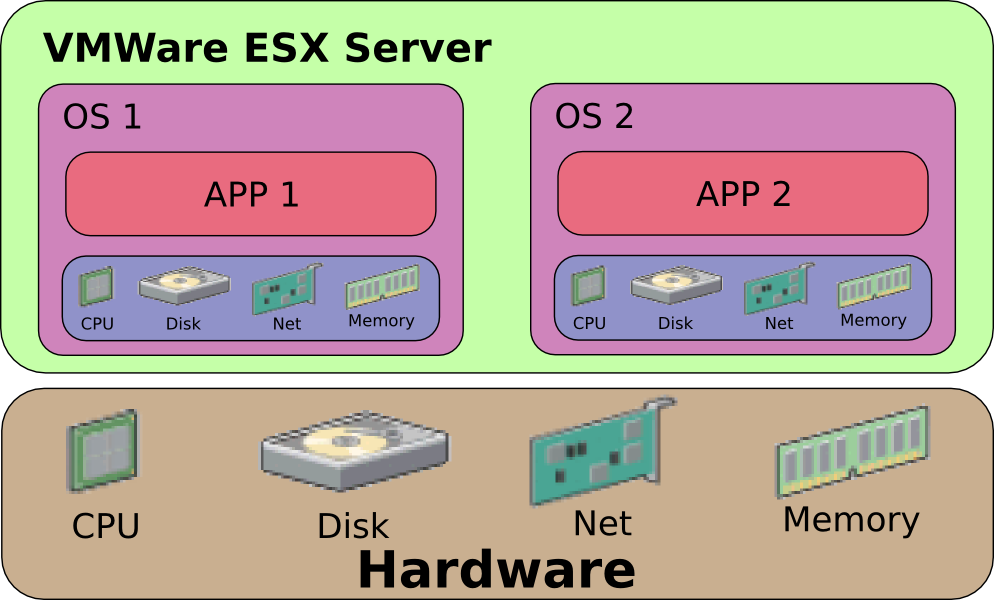
\includegraphics[width=5cm]{img/VMware-schema.png}\\
\end{description}
\end{styleframe}

\begin{styleframe}
    \frametitle{}
\begin{description}[blaat]
	\item[hypervisor] software welke runt op het host systeem en de onderliggende hardware voor quest systemen virtualiseert (beschikbaar maakt middels {\it hardware emulatie}).
	\includegraphics[width=5cm]{img/400px-Hyperviseur.png}\\
	\pause
	\item[hardware emulatie] hardware wat door het host systeem (de hypervisor) als virtuele hardware aan de guests wordt gepresenteerd.
	\pause
	\item[container] ''lichtgewicht VM..'' (later meer).
\end{description}
%\pause
%Nog wat meer termen:
%\begin{description}[blaat]
%	\item[DRS] Distributed Resource Scheduler. aan/uitschakelen hosts, migreren guests.
%	\pause
%	\item[HA] High Availability. Detecteren host failure, migreren guests.
%	\pause
%	\item [volledige ({\it full}) virtualisatie]. Alles gevirtualiseerd: guest ziet functioneel echte hardware. Best lastig in de begindagen (VMware was goed bezig (straks meer)).
%	\pause
%	\item [para virtualisatie]: de guest heeft een aangepaste kernel (Xen).
%\end{description}
\end{styleframe}

\subsection{Historie}
\begin{styleframe}
    \frametitle{Historie}
\begin{itemize}
	\item V\'o\'or virtualisatie: veel ''losse'' servers:
	\pause
	\begin{itemize}
		\item Verspilling van CPU, RAM, disk, netwerk en (niet te vergeten) power resources (bij InterNLnet ging het stroomverbruik van het datacenter met meer dan 20\% naar beneden (90\% \-> 6x\%)).
		\pause
	\end{itemize}
	\item Belangrijk (in het begin): Xen en VMware:
	\pause
	\begin{itemize}
		\item Xen: {\it para virtualisatie:} aangepaste kernel voor {\bf guest} systeem nodig.
		\pause
		\item VMware: hypervisor ESX. '{\it binary translation}': guest calls door de hypervisor vertaald (geen aangepast guest systeem nodig).
	\end{itemize}
\end{itemize}
\end{styleframe}

\subsection {}
\begin{styleframe}
    \frametitle{}
\begin{itemize}
	\item HVM (Hardware Virtual Machine). Bv. Intel VT-x en AMD-V (vanaf ca. 2006).
	\pause
	\begin{itemize}
		\item extra instructies op de CPU speciaal voor virtualisatie.
		\pause
		\item Maakte volledige virtualisatie makkelijker (juist vanwege de complexe x86 architectuur was VT-x/AMD-V erg welkom).
		\pause
		\item Tevens een enorme snelheidswinst.
		\pause
		\item Xen, VMWare, KVM, ...
		\pause
		\item Alleen voor cpu/memory. Access van netwerk en disk nog steeds via emulatie (door de hypervisor). Wel vaak via speciale drivers voor zowel guest als hypervisor (PV's: Para virtualized Drivers).
	\end{itemize}
\end{itemize}
\end{styleframe}

\subsection {Definitie virtualisatie}
\begin{styleframe}
    \frametitle{Dus wat is virtualisatie?}
\pause
Er is niet 1 definitie: erg afhankelijk van implementatie:
\pause
\begin{itemize}
	\item para?
	\item binary translation?
	\item volledig?
	\item containers?
\end{itemize}
\pause
Belangrijk dat je de terminologie en mogelijkheden kent.
\end{styleframe}

\section{KVM}
\subsection {KVM, QEMU en libvirt}
\begin{styleframe}
    \frametitle{KVM, QEMU en libvirt}
{\scriptsize
\begin{itemize}
	\item KVM:
		\begin{itemize}
			\item Onderdeel van de kernel van het host systeem.
			\pause
			\item Geen complete hypervisor.
			\pause
			\item Maakt gebruik van de hardware virtualisatie (VT-x/AMD-V). Verzorgt de mapping tussen fysieke en virtuele CPU's.
			\pause
		\end{itemize}
	\item QEMU (Quick EMUlator):
		\begin{itemize}
			\item Software op zichzelf. Emuleert hardware (ook disken, netwerk, PCI, USB, ...)
			\pause
			\item Werkt samen met KVM maar kan ook geheel zelfstandig als hypervisor dienen.
			\pause
		\end{itemize}
	\item libvirt: software voor het managen van de hypervisor en guests.
		\begin{itemize}
			\item daemon libvirtd
			\pause
			\item xml voor het definieren van VM's (en containers), netwerk, storage
			\pause
			\item cli -en grafische tools
			\pause
			\item voor KVM, QEMU, Xen, VMWare ESX, LXC, ...
			\pause
		\end{itemize}
\end{itemize}
Hypervisor is hier een combinatie van KVM en QEMU.
}
\end{styleframe}


\subsection {Installatie}
\begin{styleframefrag}
    \frametitle{Installatie}
Bijvoorbeeld voor CentOS:
\scriptsize
\begin{verbatim}
# yum -y install qemu-kvm libvirt virt-install bridge-utils
# systemctl enable libvirtd
# systemctl start libvirtd
\end{verbatim}
\end{styleframefrag}

\subsection {{\tt virsh} en virt-manager}
\begin{styleframe}
    \frametitle{virsh}
Keuze om VM's te maken/deleten etc.. uit cli ({\tt virsh}) en grafische tool ({\tt virt-manager}).
\end{styleframe}

\subsection {Virtueel netwerk}
\begin{styleframefrag}
    \frametitle{Virtueel netwerk}
VM's kunnen we een eigen virtueel netwerk geven.
Dit kan makkelijk met virt-manager.
Maar kan ook met cli en een template:
\pause
\scriptsize
\begin{verbatim}
virsh# net-list
virsh# net-list --all
virsh# net-define /root/netwerk1.xml
virsh# net-autostart netwerk1
virsh# net-start netwerk1
virsh# net-info netwerk1
\end{verbatim}
\end{styleframefrag}

\subsection{Storage pools en volumes}
\begin{styleframefrag}
    \frametitle{Storage pools en volumes}
Met libvirt kun je storage pools maken.
\begin{itemize}
	\item de default storage pool is in /var/lib/libvirt/images
	\item een storage pool bevat storage volumes (de disken)
\end{itemize}
Maak een nieuwe pool:
\scriptsize
\begin{verbatim}
# mkdir /var/lib/libvirt/pool1
# virsh
virsh# pool-define-as pool1 dir - - - - /var/lib/libvirt/pool1
(virsh# pool-define-as pool1 --type dir \
                            --target /var/lib/libvirt/pool1)
virsh# pool-autostart pool1
virsh# pool-start pool1
virsh# vol-create-as pool1 debian8.img 10G                                                                                   
\end{verbatim}
\end{styleframefrag}

\subsection {Maak een VM}
\begin{styleframefrag}
    \frametitle{Maak een VM}
\scriptsize
\begin{verbatim}
# virt-install -r 1024 --vcpus=1 -n debian8 \
    -f /var/lib/libvirt/pool1/debian8.img \
    --cdrom /home/user1/Downloads/debian-8.5.0-amd64-netinst.iso
\end{verbatim}
Enkele commando's:\\
\verb!virsh# list --all!\\
\pause
\verb!virsh# list --autostart!\\
\pause
\verb!virsh# autostart debian8!\\
\pause
\verb!virsh# destroy debian8!\\
\pause
\verb!virsh# start debian8!\\
\pause
\verb!virsh# undefine debian!\\
\pause
\verb!# virsh help | less!\\
Verkrijg het IP-adres:\\
\verb!virsh# domifaddr debian8!
\end{styleframefrag}

\begin{styleframefrag}
    \frametitle{Migreren van VM's}
\scriptsize
\pause
{\tt \# virsh destroy ''name\_of\_vm''}\\
\pause
{\tt \# virsh destroy ''name\_of\_vm''}\\
\pause
{\tt \# scp /tmp/''vmname''.xml ''hostX:''}\\
\pause
{\tt \# scp /var/lib/libvirt/images/''vmname''.img ''hostX:''}\\
\pause
~\\
Op de ''hostX'': verwijder uuid's in xml-file.\\
\pause
{\tt hostX:\# virsh define ''vmname''.xml}\\
\pause
{\tt hostX:\# virsh start ''vmname''}\\
\pause
\end{styleframefrag}

\section{Conlusies}
\subsection {Hypervisor vs container}
\begin{styleframe}
    \frametitle{Hypervisor vs container}
De functie van de hypervisor is wat bleekjes tegenwoordig. Enkele nadelen:
\pause
\begin{itemize}
    \item Netwerk/disk access via ''paravirtualized drivers'' (PV drivers). Verschillende PV-drivers nodig per hypervisor (VMware's ESX, Xen, KVM) \'en per guest OS (windows 7, windows 10, redhat, ubuntu etc..) \-> veel code!
    \pause
    \item OS-patching in je VM's!
    \pause
    \item Relatief veel resources nodig per VM (vergeleken met containers).
    \pause
%    \item DRS en HA niet meer zo'n USP's: er komen steeds meer ''container management'' tools zoals bv. ''Kubernetes''.
    \item management niet meer zo'n USP's: er komen steeds meer ''container management'' tools zoals bv. ''Kubernetes''.
    \pause
    \item Security is ook sterk verbeterd mbt containers. Zeker sinds de extra instructies op de CPU (VT-x/AMD-V).
    \pause
    \item Een hypervisor is goed in het ondersteunen van een hybride omgeving (verschillende OS\-sen). Maar wat is het voordeel daarvan?
\end{itemize}
\end{styleframe}

\subsection {Kubernetes}
\begin{styleframe}
    \frametitle{}
We kijken dan ook niet alleen naar de ''gewone'' (hypervisor) virtualisatie (met KVM) maar ook naar containers:
\pause
\begin{itemize}
    \item Vandaag: KVM (+ QEMU en libvirt)
    \pause
    \item Volgende keer: containers (docker)
    \pause
    \item Daarna: Kubernetes (..)
\end{itemize}
\end{styleframe}

